% KWEB Del 1.1 (WP1.1) Report
%

\documentclass[a4paper,twoside,12pt]{report}
\usepackage{times}
\usepackage{graphics}
%\usepackage{graphicx}
%\usepackage{epsfig}
%\usepackage[]{graphicx}
\usepackage{deliverable}
%\usepackage{pnamed}

%cabeceras

\usepackage[T1]{fontenc}
% españolización
\usepackage[english]{babel}
\usepackage[utf8]{inputenc}
\usepackage{rotating}
\usepackage{graphicx}
\usepackage{color}
\usepackage{xspace}
% mejoras visuales
\usepackage{enumerate}
\usepackage{fancyhdr}  % para configurar los encabezados
\usepackage{fancybox}  % para hacer cajitas
\usepackage[normal,oneline,sf,bf]{caption2}
\usepackage{titlesec}  % para configurar los títulos de sección
\usepackage{paralist}
\usepackage{url}
\usepackage{latexsym}
\usepackage{amsmath}
\usepackage{amssymb}
\usepackage{amsthm}

\usepackage{epigraph}

% citas, referencias e índices
\usepackage{cite}
%\usepackage{citesort}   % da errores al compilar
\usepackage{makeidx}

% incrustaciones de código fuente
%\usepackage[norules,nolineno]{lgrind}
\usepackage{verbatim}
\usepackage{listings}
%\usepackage{noweb,a4wide}


%\usepackage{textcomp}
\usepackage[right]{eurosym}

% columnas
\usepackage{multicol}

% tablas
\usepackage{longtable}

%\input{commands}

% \addto\captionsspanish{
%         \def\listtablename{\'Indice de tablas}%
%         \def\tablename{Tabla}} 



\lstset{%
        language=Java,
	basicstyle=\footnotesize\sffamily,
	keywordstyle=\bfseries, %\color{darkred}
 	stringstyle=\itshape, %\color{violet}
 	commentstyle=\itshape, %\color{blue}
 	showspaces=false,
 	showtabs=false,
 	showstringspaces=false,
 	frame=trBL,
        frameround=tttt,
        %backgroundcolor=\color{lightyellow},
 	extendedchars=true,
 	numbers=none,
        aboveskip=0.5cm,
        belowskip=0.5cm,
        xleftmargin=1cm,
        xrightmargin=1cm,
	breaklines=true,
        morekeywords={PREFIX,java,rdf,rdfs,url,dcterms,foaf,skos,gr,skosxl}
}
\definecolor{darkred}{rgb}{0.5, 0, 0}
\definecolor{violet}{rgb}{1, 0, 1}
\definecolor{lightyellow}{rgb}{1,1,0.8}


\newtheorem{theorem}{Theorem}[section]
\newtheorem{proposition}[theorem]{Proposición}
\newtheorem{lemma}[theorem]{Lema}
\newtheorem{definition}[theorem]{Definición}
\newtheorem{examples}[theorem]{Ejemplo}
\newtheorem{remarks}[theorem]{Remarks}
\newtheorem{corollary}[theorem]{Corolario}
\newtheorem{remark}[theorem]{Remark}
\newtheorem{example}[theorem]{Ejemplo}
\newtheorem{conjecture}[theorem]{Conjecture}
\newtheorem{note}[theorem]{Nota}



\begin{document}

\title{Quality Management in Service-based Systems and Cloud Applications}

\author{
{Jose María Alvarez-Rodríguez (SEERC)\\
jmalvarez@seerc.org \\
josem.alvarez@josemalvarez.es}}

\revised{September 30, 2013}

\issuer{Jose María Alvarez-Rodríguez}

\identifier{WP4-SEERC-ER-TR}

\version{v1.0}

\state{Final}

\project{WP4 Quality Management and Business Model Innovation}

\distribution{protected}

\synopsis{\strut\\
% Cloud Computing and Service Oriented Architectures have seen a dramatic increase of the amount of applications, 
% services, management platforms, data, etc. gaining momentum the necessity of new complex methods 
% and techniques to deal with the vast heterogeneity of data sources or services. In this sense Quality of Service (QoS) 
% seeks for providing an intelligent environment of self-management components based on domain knowledge in which 
% cloud components can be optimized easing the transition to an advanced governance environment. On the other hand, 
% semantics and ontologies have emerged to afford a common and standard data model that eases the interoperability, integration and 
% monitoring of knowledge-based systems. Taking into account the necessity of an interoperable and intelligent system to manage QoS in 
% cloud-based Systems and the emerging application of semantics in different domains, this paper reviews the main approaches for 
% semantic-based QoS management as well as the principal methods, techniques and standards for processing and exploiting diverse data 
% providing advanced real-time monitoring services. A semantic-based framework for QoS management is also outlined taking advantage of 
% semantic technologies and distributed datastream processing techniques. Finally a discussion of existing efforts and challenges are 
% also provided to suggest future directions.\\

Technical Report.


Keywords: cloud computing, services quality, semantics
}

\coverpages

\setcounter{page}{0}

\pagenumbering{roman}

% \include{historial}
% \include{resumen}

\setlength{\parskip}{0.0cm}
\tableofcontents
\listoffigures
\listoftables
\setlength{\parskip}{1.0ex}

\newpage
\pagenumbering{arabic}


%%%%%%%%%%%%%%%%%%%%%%%%%%%%%%
% \pagestyle{kweb}
\chapter{Introduction}
Cloud Computing~\cite{mell2011nist} systems and Service Oriented Architectures (SOA) have 
reached a level of complexity~\cite{Huebscher:2008:SAC:1380584.1380585,Conejero:2012:MSQ:2357487.2357591} that implies the necessity of new methods 
and algorithms to automatically deal with the vast amount of data, variables, 
parameters, etc. that appears in this new realm for the advanced management of 
applications, services or resources. 

In this new environment QoS is playing a relatively minor role but its 
importance, in a wide range of applications scenarios, is likely become more 
crucial than ever before. In recent years and due to the deployment of web 
services a considerable research effort in QoS has been made. However existing 
QoS mechanisms are actually available in a few large scale commercial 
environments and with a limited extent. The main problem lies in the complexity 
of designing QoS models that enables an adequate management of a distributed 
architecture making decisions about resource provisioning, getting feedback for 
the final users, etc. with the objective of avoiding existing ``brute-force''
solutions and overprovisioning. 

Although QoS management has been also widely investigated~\cite{Conejero:2012:MSQ:2357487.2357591} 
in the well-known grid-computing area the emergence of the Cloud Computing paradigm 
brings a new set of open issues: accomplish the  Service Level Agreements (SLAs), predict 
future workload, process large and diverse data streams/logs, make real-time 
decisions, reasoning and inference, dynamic adaptation and provision of 
resources, etc. In the widely-accepted definition~\cite{mell2011nist} of 
he National Institute of Standards and Technology (NIST) QoS 
would be aligned to the concept of ``Measured Service'', see Figure~\ref{fig:qos-intro}, and more specifically to define both characteristics applicable to a service and operations 
to be delivered such as predictive analysis. The aforementioned points are very challenging and should be 
addressed in order to ease an intelligent, flexible and self-managing system of cloud-based applications and platforms.

% 
 \begin{figure}[!ht]
\centering
	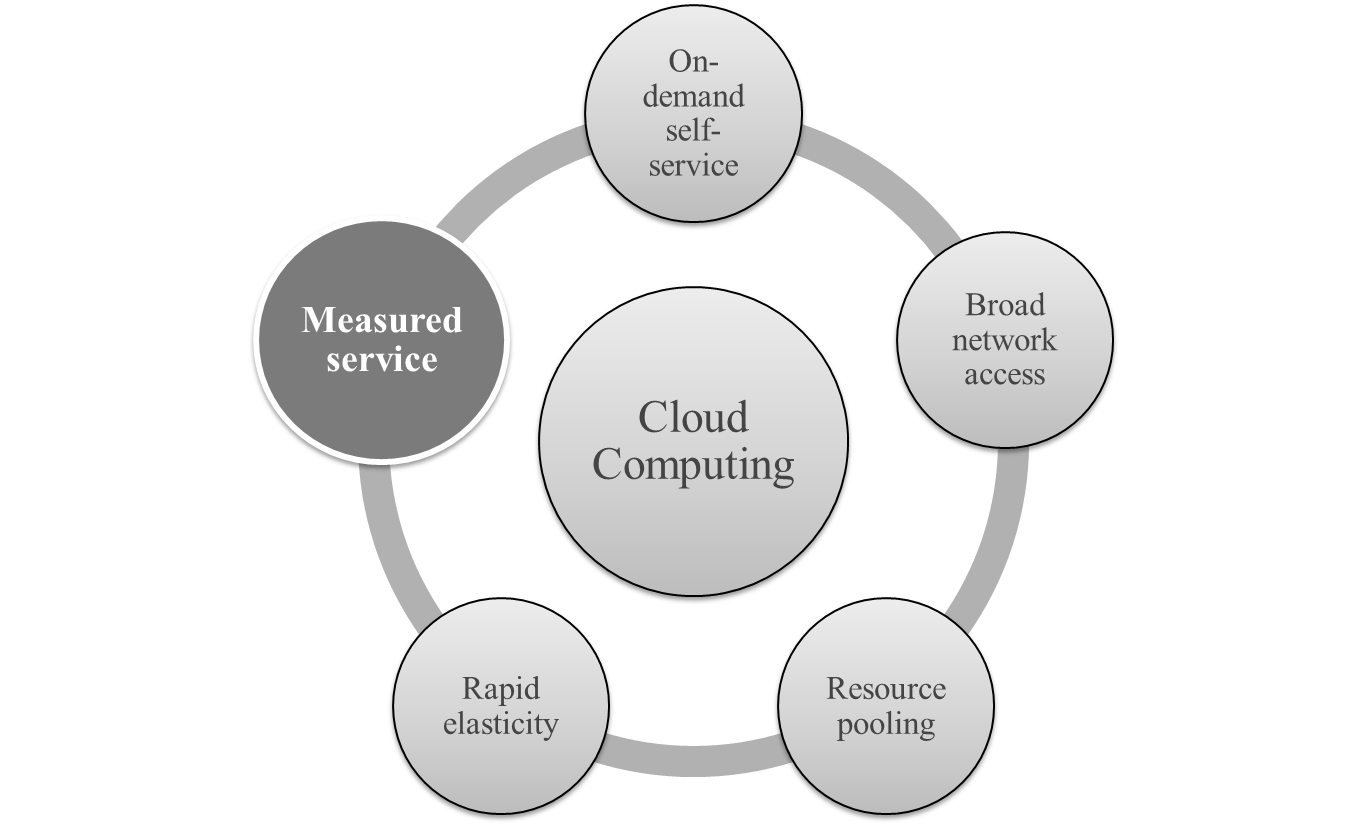
\includegraphics[width=12cm]{./imgs/qos-intro}
 \caption{Quality of Service in the NIST definition~\cite{mell2011nist}.}
 \label{fig:qos-intro}
\end{figure}

Furthermore a proper management of a cloud system taking into account QoS 
features can save costs, keep high-performance, reserve resources on-demand and 
offer a user-friendly experience to both IT managers and final users. 
Traditionally, QoS has been handled using a combination of network resource 
provisioning with techniques such as admission control or active queue 
management. Nowadays these old-fashioned techniques can be applied to a static 
environment but in the near future with the new implications for professionals~\cite{DBLP:journals/jucs/Colomo-PalaciosFSS12}, 
the challenge of providing higher elasticity and dynamic adaptation cannot be accomplished with these methods. In this sense it is clear that QoS will remain a fundamental requirement in the next wave of 
applications and services on the Web and there is no doubt that QoS should 
address the new challenges applying emerging and trending technology and 
approaches to overcome existing restrictions in QoS models.

The features and requirements of these new cloud systems with regards 
to QoS~\cite{Pedersen:2011:AMQ:2114495.2115542} and their implications in the future IT~\cite{DBLP:journals/jucs/Colomo-PalaciosFSS12} 
match the advantages of software component and knowledge-based architectures. In fact, Autonomic Computing support for the next generation of cloud systems 
needs to be~\cite{Conejero:2012:MSQ:2357487.2357591,Pedersen:2011:AMQ:2114495.2115542}: 
1) Self-x management, 2) agile, flexible and reliable, 4) deployable over a multiple cloud platforms, 5) handle complexity, 6) enable 
collaboration and coordination and 7) cost-effective and greener 
(energy-efficient). Under this context, semantic technologies have emerged as an 
option to design and develop intelligent software components and agents to 
perform certain tasks on the Web and fulfill user's requirements (in this case 
applications). Therefore, Semantics enables machines to automatically process 
and enrich data from different sources and has the potential to deeply influence 
the further development of the Internet Economy as cloud systems also does.

In the Semantic Web area, there is a growing commitment to process large data streams applying 
new stream reasoning~\cite{Bolles:2008:SSE:1789394.1789438,Barbieri:2010:EEC:1739041.1739095} 
or complex event processing~\cite{Anicic:2011:EUL:1963405.1963495} (CEP) techniques. Furthermore there are research works offering cloud-based 
solutions to deal with Big Data~\cite{Fan:2013:MBD:2481244.2481246} (e.g. analysis of social media), modeling SLAs and ECA rules with ontologies, 
monitoring real-time systems (e.g. traffic), sensor networks, or making decisions in a collaborative fashion~\cite{RodriGuez-GonzaLez:2012:UAP:2350799.2350907} (e.g. clinical reasoning). 
The main advantage of applying semantic technologies to a specific domain lies in the standard representation of knowledge and data through a common-shared data model (RDF) and the 
capacity of reusing existing knowledge through ontologies (OWL). Thus, data coming from cloud systems can be automatically processed, checked for inconsistencies and 
used in expert systems to support self-x management activities.

This review is intended to provide researchers, developers and practitioners a summary of the current status of QoS management in Cloud Computing and SOA applying semantics. To do so, the paper 
is structured as follows. Next section reviews the background concepts required to a better understanding of the paper. Section~\ref{qos-semantics} 
presents the existing works to perform QoS management using semantics; more specifically most of the ontology-based frameworks for 
QoS management are reviewed. Afterwards, a review of existing techniques for processing large data streams is also provided in Section~\ref{data-stream}. 
Section~\ref{framework} outlines a framework to meet QoS requirements applying semantics and data stream processing techniques in real-time. 
Finally, the paper ends with a discussion of existing approaches for semantic-based QoS management, 
limitations, future challenges and concluding remarks. 


This chapter presents a brief summary of the background concepts reviewed in this paper: 
1) Cloud Computing and QoS; 2) Semantic Technologies and 3) Big Data, with the 
aim of building a common understanding of the requirements of QoS in Cloud Computing.
\section{Quality of Service in Cloud Systems}\label{qos-cloud-index}
Cloud Computing represents the next natural step in the evolution of on-demand services and applications. 
Several definitions have been made but the description~\cite{mell2011nist} provided by the NIST institute has reached a major consensus:  
\textit{A large-scale distributed computing paradigm that is driven by economies of scale, in which a pool of 
abstracted, virtualized, dynamically-scalable, managed computing power, storage, platforms, and services are delivered on demand to external customers over the Internet}. 
The NIST institute has also defined~\cite{mell2011nist}: 
\begin{enumerate}
 \item Five key characteristics: on-demand self-service, ubiquitous network access, location independent resource pooling, rapid elasticity and pay per use.
 \item Three service models: Software-as-a-Service (SaaS), Platform-as-a-Service (PaaS) and Infrastructure-as-a-Service (IaaS).
 \item Four development models: private, community, public and hybrid clouds. 
\end{enumerate}

These basic concepts~\cite{mell2011nist} and usages~\cite{cloud-usage} in a cloud environment lead us to consider that QoS is a key-enabler of the five essential characteristics identified by 
the NIST institute and it is closely related to the concepts of Autonomic and Utility Computing~\cite{Huebscher:2008:SAC:1380584.1380585}. 
As a consequence the QoS management must play a major role in cloud environments and in the Future Internet to 
afford, from a quality point of view, the implementation of the ``Measured Service'' concept, see Figure~\ref{fig:qos-intro}.

On the other hand, the ITUT-T Recommendation E.800 defines QoS as \textit{collective effect of service performance that determines the degree of 
satisfaction by a user of the service}. Thus QoS data is a key-enabler to design, identify and put in action SLAs. It should also influence 
software components and applications to ensure a reliable environment for executing services. Some open issues in 
QoS management emerge to extend this definition including reputation-based mechanisms for service selection or 
dynamic adaptation of resource provisioning. The application of QoS has been widely studied and 
applied~\cite{Conejero:2012:MSQ:2357487.2357591,Pedersen:2011:AMQ:2114495.2115542} to web services and grid computing areas and it is now 
gaining momentum in the new Cloud Computing paradigm. 

In order to facilitate the QoS management in the cloud-environment some tools, called Cloud Management Platforms (CMPs) can be found 
to manage the different layers of cloud-based applications but the majority of them are now focused on the IaaS and PaaS layers. 
The use of these platforms can help to manage the growing of cloud applications and ease the deployment and monitoring of services across 
public and private clouds. The six key capabilities~\cite{Kephart2012} that we should look for in a CMP are: simplify complexity, 
manage multiple clouds, build for the future, support the whole application lifecycle, self-management (set-it and forget-it) and manage/control costs. 
In this sense OASIS just launched a CAMP TC to create and inter-operable protocol that cloud 
implementers can use to package and deploy their applications. The idea is to provide a set of REST services, at the PaaS layer, to foster an ecosystem of 
common tools, plug-ins, libraries and frameworks, which will allow vendors to offer greater value-add. In the particular case of QoS, the use of standards to gather data 
from applications can improve the process of making decisions about resource provisioning or help in saving costs among others. Nevertheless 
this specification is still in an early stage and its objectives are more focused on the management of cross-cloud applications than a 
real management from QoS point of view. Following main characteristics of the CAMP specification are presented:
\begin{itemize}
 \item It is a language, framework and platform neutral to manage in the same way Java, Ruby on Rails or Node.js applications.
 \item It only covers interactions between a cloud consumer and a provider~\cite{mell2011nist}.
 \item It supports the management of the entire lifecycle of the application not just the deployment of isolated components.
 \item A major objective of the specification is to provide an inter-operable environment. They are trying to keep simple as 
 possible but with the possibility of being extended by third-parties.
\end{itemize}

Although there is no a clear objective to support quality indicators it can be considered as a major effort to unify information exposed by providers and 
improve the creation of an integrated and inter-operable ecosystem in which existing cloud management application platforms such 
as RightScale, Enstratus, ScaleUp, Cloudability, Cloudyn, CloudExpress or MyGravitant can take advantage of implemented 
added-value services on the top of a common API. Although these commercial products offer a very good option 
to manage cloud-based applications there is a lack of standardization and some QoS features cannot be managed.  
Nevertheless these existing cloud management platforms present some interesting features and services for 
multi-cloud management that must be taken into account in the design of a dedicated cloud quality management platform such as:
\begin{itemize}
 \item Integrated management of cloud resources: compute, networking and storage.
 \item Organization: tagging capabilities or creation of profiles and views to group cloud resources.
 \item Accessibility and usability: monitoring (tracking and graphing custom metrics), dashboard or import capabilities.
 \item Custom services: creation of alerts using a particular set of indicators, cost forecasting or reporting.
\end{itemize}

%Policy making
On the other hand there is an interesting approach to manage cloud quality indicators using a policy-making 
perspective. In this sense public and private bodies are continuously seeking for new analytical tools and methods to 
assess, rank and compare their performance based on distinct indicators and dimensions with the objective of making 
some decision or developing a new policy. In this context the creation and use of quantitative indexes is 
a widely accepted practice that has been applied to various domains such as Bibliometrics and academic performance and 
quality (the Impact Factor by Thomson-Reuters, the H-index or the Shanghai and Webometrics rankings) the Web impact (the Webindex~\cite{webindexlod} 
by the Webfoundation) or Smart Cities (The European Smart Cities ranking) to name a few. Therefore policymakers as well as individuals are 
continuously evaluating quantitative measures to tackle or improve existing problems in different areas and 
support their decisions. Nevertheless the sheer mass of data now available is raising a new dynamic and challenging environment 
in which traditional tools are facing major problems to deal with data-sources diversity, structural issues or complex processes of estimation. 
According to some efforts such as the ``Policy-making $2.0$'' within the Cross-Over project~\footnote{\url{http://www.crossover-project.eu/}} 
that \textit{refers to a blend of emerging and fast developing technologies that enable better, more timely and more participated decision-making}, 
new paradigms and tools are required to take advantage of the existing environment (open data and big data) to design and estimate 
actions in this dynamic context according to requirements of transparency, standardization, adaptability and extensibility among 
others with the aim of providing new context-aware and added-value services such as visualization that 
can help a deepen and broaden understanding of the impact of a policy in a more fast and efficient way. 
As a consequence common features and requirements can be extracted from the existing situation out:
\begin{itemize}
 \item Data sources. Data and information is continuously being generated as observations from social networks, public and private institutions, NGOs, services and applications, etc. 
 creating a tangled environment of sources, formats and access protocols with a huge but restricted potential for exploitation. Nevertheless data processing, knowledge inferring, etc. are not mere processes 
 of gathering and analyzing, it is necessary to deal with semantic and syntactic issues, e.g. particular measurements and dimensions or name mismatches, 
 in order to enable a proper data/information re-use and knowledge generation.
 
 \item Structure. Quantitative indexes are usually defined (a mathematical model) by experts to aggregate several indicators (in a hierarchy structure) 
 in just one value to provide a measure of the impact or performance of some policy in a certain context. The structure of these indexes are 
 obviously subjected to change over time  to collect more information or adjust their composition and relationships (narrower/broader). 
 That is why technology should be able to afford adequate techniques to automatically populate new changes in an efficient way.
 
  \item Computation process. This feature refers to the calculation of the index. Observations are gathered from diverse data sources and aligned 
  to the index structure, commonly indicators, that are processed through various mathematical operators to generate a final index value. 
  Nevertheless the computation process is not always described neither open (any minor change can imply a long time for validation) implying that 
  cannot be easily replied for third-parties with other purposes, for instance research, preventing one 
  of the most wanted characteristics such as transparency. Furthermore it is necessary to ensure that the computation process 
  is sound and correct.

  \item Documentation. As the European project Cross-over has stated, new policy-making strategies go ahead of a simple and closed value and it is necessary to bring 
  new ways of exploiting data and information. Moreover the use of the Web as a dissemination channel represents a powerful environment in which 
  information should be available taking into account the multilingual and multicultural character of information. In this context documentation mechanisms 
  must necessarily cover all the aforementioned features to afford a detailed explanation of a quantitative index-based policy to both policymakers 
  and final users. However existing initiatives usually generates some kind of hand-made report which is not easy to keep up-to-date and deliver 
  to the long-tail of interested third-parties.
\end{itemize}

Following this perspective of creating a quantitative index the Cloud Computing community~\cite{Maiya:2012:QMC:2353730.2353862,DBLP:conf/quatic/KlemsBW12} 
and some of the big players have launched some relevant indexes such as:

\begin{itemize}
 \item The Service Measurement Index (SMI) by the Cloud Services Measurement Initiative Consortium (CSMIC) consortium. It is 
 based on a framework of critical key performance indicators (both business and technical) \textit{associated attributes, and measures 
 that provide a standardized method for measuring and comparing a business service regardless of whether that service is internally provided or sourced from an outside company for any cloud service (IaaS, PaaS, SaaS, etc.). It is designed to become a 
 standard method to help organizations measure cloud-based services based on their specific business and technology requirements.} As 
 an implementation of the SMI Index the ``Ranking Clouds''~\cite{DBLP:journals/fgcs/GargVB13} presents a framework to manage this index 
 and makes a ranking of different PaaS providers using the Analytic Hierarchy Process (AHP) method to weight some key performance indicators.
 
 \item The Cisco Global Cloud Index (GCI) by Cisco. \textit{It is an ongoing effort to forecast the growth of global data 
 center and cloud-based IP traffic. The forecast includes trends associated with data center virtualization and cloud computing. }
 It also provides a visual representation of countries ranging  from ``Cloud Prepared'' to ``Cloud Emerging''.

 \item The CSC Cloud Usage index. It is an index created through a survey of more than $3500$ cloud computing users 
 in eight countries around the world. The survey is focused on capturing user information about outcomes and 
 experiences rather than predictions and intentions.

 \item The VMWare Cloud index. It is an study conducted by Forrester Consulting and ITR in Japan. \textit{The 2012 study surveyed 
 approximately $6500$ senior IT practitioners across the APJ region in eleven countries / regions with the aim of establishing 
 top cloud drivers and concerns in the community.}

\end{itemize}

As final remark, the creation of a quantitative index of QoS indicators seems to be a promising approach because 
it represents a joint effort to establish a common set of KPI's and it can be applied to the different cloud types and models. Furthermore 
the participation of big players validates and ensures their potential development. Nevertheless, as other existing quantitative indexes, 
the structure and the computing process are completely closed and there is not any framework to automatically compute observations. Apart from 
that it would also be necessary the definition of an API for exposing quality indicators that could be part of existing CAMPs.

% 
% 
% \begin{sidewaystable}[!ht]
% \renewcommand{\arraystretch}{1.3}
% \tiny
% \begin{center}
% \begin{tabular}[c]{|p{2.5cm}|p{9cm}|p{1.5cm}|p{1.5cm}|p{1.5cm}|} 
% \hline
%   \textbf{KPI} &  \textbf{Definition}  &  \textbf{Broader} & \textbf{Defined by} & \textbf{Scope} \\\hline
%   Accountability&This component is used to measure the properties related to the service provider
% organization. These properties may be independent of the service being provided.&&CSMIC&$\ast$ \\ \hline
%   Agility&Indicates the impact of a service upon a client's ability to change direction, strategy, or tactics quickly and with minimal disruption.&&CSMIC&$\ast$ \\ \hline
%   Assurance&This category includes key attributes that indicate how likely it is that the service will be available as specified.&&CSMIC&$\ast$ \\ \hline 
%   Financial&The amount of money spent on the service by the client.&&CSMIC&$\ast$ \\ \hline 
%   Performance&This category covers the features and functions of the provided services.&&CSMIC&$\ast$ \\ \hline 
%   Security and Privacy&This category includes attributes that indicate the effectiveness of a service provider's controls on access to services, service data, and the physical facilities from which services are provided.&&CSMIC&$\ast$ \\ \hline 
%   Usability&The ease with which a service can be used.&&CSMIC&$\ast$ \\ \hline 
%   Auditability&The ability of a client to verify that the service provider is adhering to the standards, processes, and policies that they follow.&Accountability&CSMIC&$\ast$ \\ \hline 
%   Compliance&Standards, processes, and policies committed to by the service provider are followed.&Accountability&CSMIC&$\ast$ \\ \hline 
%   Contracting Experience&Indicators of client effort and satisfaction with the process of entering into the agreements required to use a service.&Accountability&CSMIC&$\ast$ \\ \hline 
%   Data Ownership&The Level of rights a client has over client data associated with a service.&Accountability&CSMIC&$\ast$ \\ \hline 
%   Ease of Doing Business&Client satisfaction with the ability to do business with a service provider.&Accountability&CSMIC&$\ast$ \\ \hline 
%   Ease of Doing Business&The processes used by the service provider to manage client expectations, issues and service performance.&Accountability&CSMIC&$\ast$ \\ \hline 
%   Ownership&The level of rights a client has over software licenses, intellectual property and data associated with a service.&Accountability&CSMIC&$\ast$ \\ \hline 
%   Provider business stability&The likelihood that the service provider will continue to exist throughout the contracted term.&Accountability&CSMIC&$\ast$ \\ \hline 
%   Provider Certifications&The service provider maintains current certifications for standards relevant to their clients' requirements.&Accountability&CSMIC&$\ast$ \\ \hline 
%   Provider Contract/SLA Verification&The service provider makes available to clients SLAs adequate to manage the service and mitigate risks of service failure.&Accountability&CSMIC&$\ast$ \\ \hline 
%   Provider Ethicality&Ethicality refers to the manner in which the service provider conducts business; it includes business practices and ethics outside the scope of regulatory compliance. Ethicality includes fair practices with suppliers, customers, and employees.&Accountability&CSMIC&$\ast$ \\ \hline 
%   Provider Personnel Requirements&The extent to which service provider personnel have the skills, experience, education, and certifications required to effectively deliver a service.&Accountability&CSMIC&$\ast$ \\ \hline 
%   Provider Supply Chain&The service provider ensures that any SLAs that must be supported by its suppliers are supported.&Accountability&CSMIC&$\ast$ \\ \hline 
%   Security Capabilities&The capabilities of service providers to ensure application, data, and infrastructure securiy based on the security requirements of the client.&Accountability&CSMIC&$\ast$ \\ \hline 
%   Sustainability&The impact on the economy, society and the environment of the service provider.&Accountability&SMIC&$\ast$ \\ \hline 
%   Adaptability&The ability of the service provider to adjust to changes in client requirements.&Agility&CSMIC&$\ast$ \\ \hline 
%   Capacity&The maximum amount of a service that a service provider can deliver while meeting agreed SLAs.&Agility&CSMIC&$\ast$ \\ \hline 
%   Elasticity&The ability of a service to adjust its resource consumption to meet demand.&Agility&CSMIC&$\ast$ \\ \hline 
%   Extensibility&The ability to add new features or services to existing services.&Agility&CSMIC&$\ast$ \\ \hline 
%   Flexibility&The ability to add or remove predefined features from a service.&Agility&CSMIC&$\ast$ \\ \hline 
%   Portability&The ability of a client to easily move a service from one service provider to another with minimal disruption.&Agility&CSMIC&$\ast$ \\ \hline 
%   Scalability&The ability of a service provider to increase or decrease the amount of service available to meet client requirements.&Agility&CSMIC&$\ast$ \\ \hline 
% \hline
% \end{tabular}
% \caption{Key Performance Indicators I.}\label{table:kpi-1}
%   \end{center}
% \end{sidewaystable} 
% 
% \begin{sidewaystable}[!ht]
% \renewcommand{\arraystretch}{1.3}
% \tiny
% \begin{center}
% \begin{tabular}[c]{|p{2.5cm}|p{9cm}|p{1.5cm}|p{1.5cm}|p{1.5cm}|} 
% \hline
%   \textbf{KPI} &  \textbf{Definition}  &  \textbf{Broader} & \textbf{Defined by} & \textbf{Scope} \\\hline
%  Availability&The amount of time that a client can make use of a service.&Assurance&CSMIC&$\ast$ \\ \hline 
%  Maintainability&Maintainability refers to the ability for the service provider to make modifications to the service to keep the service in a condition of good repair.&Assurance&CSMIC&$\ast$ \\ \hline 
%  Recoverability&Recoverability is the degree to which a service is able to quickly resume a normal state of operation after an unplanned disruption.&Assurance&CSMIC&$\ast$ \\ \hline 
%  Reliability&Reliability reflects measures of how a service operates without failure under given conditions during a given time period.&Assurance&CSMIC&$\ast$ \\ \hline 
%  Resiliency&The ability of a service to continue to operate properly in the event of a failure in one or more of its components.&Assurance&CSMIC&$\ast$ \\ \hline 
%  Stability&The degree to which the service is resistant to change, deterioration, or displacement.&Assurance&CSMIC&$\ast$ \\ \hline 
%  Serviceability&The ease and efficiency of performing maintenance and correcting problems with the service.&Assurance&CSMIC&$\ast$ \\ \hline 
%  Acquisition&Any client costs to acquire the rights and ability to use a service and to move from an existing service to the new one.&Financial&CSMIC&$\ast$ \\ \hline 
%  On-going Cost&The client cost to operate a service. This includes both recurring flat costs (e.g. monthly access fees) and usage-based costs.&Financial&CSMIC&$\ast$ \\ \hline 
%  Profit&Arrangement between client and provider(s) under which costs or profits of a service are shared by the involved parties, according to an agreed upon formula.&Financial&CSMIC&$\ast$ \\ \hline 
%  Accuracy&The extent to which a service adheres to its requirements.&Performance&CSMIC&$\ast$ \\ \hline 
%  Functionality&The specific features provided by a service.&Performance&CSMIC&$\ast$ \\ \hline 
%  Suitability&How closely do the capabilities of the service match the needs of the client.&Performance&CSMIC&$\ast$ \\ \hline 
%  Suitability&How closely do the capabilities of the service match the needs of the client.&Usability&CSMIC&$\ast$ \\ \hline 
%  Suitability&The ability of a service to easily interact with other services (from the same service provider and from other service providers).&Performance&CSMIC&$\ast$ \\ \hline 
%  Service Response Time&An indicator of the time between when a service is requested and when the response is available.&Performance&CSMIC&$\ast$ \\ \hline 
%  Access Control&Policies and processes in use by the service provider to ensure that only the provider and client personnel with appropriate status/reasons to make use of or modify data/work products may do so.&Security and Privacy&CSMIC&$\ast$ \\ \hline 
%  Geographical Constraint&The client's constraints on service location based on geography.&Security and Privacy&CSMIC&$\ast$ \\ \hline 
%  Political Constraint&The client's constraints on service location based on politics.&Security and Privacy&CSMIC&$\ast$ \\ \hline 
%  Data Integrity&Keeping the data that is created, used, and stored in its correct form so that clients may be confident that it is accurate and valid.&Security and Privacy&CSMIC&$\ast$ \\ \hline 
%  Data Privacy&Client restrictions on access and use of client data are enforced by the service provider. Any failures of these protections are promptly detected and reported to the client.&Security and Privacy&CSMIC&$\ast$ \\ \hline 
%  Data Loss&Client restrictions on access and use of client data are enforced by the service provider. Any failures of these protections are promptly detected and reported to the client.&Security and Privacy&CSMIC&$\ast$ \\ \hline 
%  Physical \& Environmental Security&Policies and processes in use by the service provider to protect the provider facilities from unauthorized access, damage or interference.&Security and Privacy&CSMIC&$\ast$ \\ \hline 
%  Proactive Threat \&  Vulnerability Management&Mechanisms in place to ensure that the service is protected against know recurring threats as well as new evolving vulnerabilities.&Security and Privacy&CSMIC&$\ast$ \\ \hline 
%  Retention/Disposition&The service provider’s data retention and disposition processes meet the clients' requirements.&Security and Privacy&CSMIC&$\ast$ \\ \hline 
%  Accessibility&The degree to which a service is operable by users with disabilities.&Usability&CSMIC&$\ast$ \\ \hline 
%  Client Personnel Requirements&The minimum number of personnel satisfying roles, skills, experience, education, and certification required of the client to effectively utilize a service.&Usability&CSMIC&$\ast$ \\ \hline 
%  Client Personnel Requirements&Installability characterizes the time and effort required to get a service ready for delivery (where applicable).&Usability&CSMIC&$\ast$ \\ \hline 
%  Learnability&The effort required of users to learn to use the service.&Usability&CSMIC&$\ast$ \\ \hline 
%  Operability&The ability of a service to be easily operated by users.&Usability&CSMIC&$\ast$ \\ \hline 
%  Transparency&The extent to which users are able to determine when changes in a feature or component of the service occur and whether these changes impact usability.&Usability&CSMIC&$\ast$ \\ \hline 
%  Understandability&The ease with which users can understand the capabilities and operation of the service.&Usability&CSMIC&$\ast$ \\ \hline 
% 
% \hline
% \end{tabular}
% \caption{Key Performance Indicators II.}\label{table:kpi-2}
%   \end{center}
% \end{sidewaystable} 
% 

\section{Semantic Technologies}
The Semantic Web area, coined by Tim Berners-Lee in 2001, has experienced recent times a growing 
commitment from both academia and industrial areas  with the objective of elevating the meaning of web 
information resources through a common and shared data model (graphs) and an underlying semantics based 
on different logic formalisms (ontologies). The Resource Description Framework (RDF), based on a graph model, and the Web Ontology Language (OWL), 
designed to formalize and model domain knowledge, are the two main \textit{ingredients} to reuse information and data 
in a knowledge-based realm. Thus data, information and knowledge can be easily shared, exchanged and linked~\cite{Maali_Cyganiak_2011} 
to other knowledge-based systems and databases through the use URIs, more specifically HTTP-URIs. Therefore the broad objective of this effort can be summarized 
as a new environment of added-value information and services that can boost and improve B2B (Business to Business), B2C (Business to Client) or 
A2A (Administration to Administration) relationships. The implementation of new context-awareness expert systems to tackle existing 
cross-domain problems such as medical reasoning, analysis of social media, etc. in which data heterogeneities, 
lack of standard knowledge representation and interoperability problems are common factors that the use of semantics can improve. As a practical view of the Semantic Web, 
the Linked Data~\cite{Heath_Bizer_2011} initiative emerges to create a large and distributed database on the Web. 
In order to reach this major objective the publication of information and data under a common data model (RDF) 
with a specific formal query language (SPARQL) provides the required building blocks to turn the Web of documents 
into a real database or ``Web of Data''. Research works are focused in two main areas: 1) production/publishing~\cite{bizer07how} and 2) consumption of 
Linked Data. In the first case data quality~\cite{Bizer2009QA}, conformance~\cite{DBLP:journals/ws/HoganUHCPD12}, 
provenance~\cite{w3c-prov} and trust, description of datasets~\cite{void} and entity reconciliation~\cite{Maali_Cyganiak_2011} issues are becoming major objectives since a mass of amount data is already available through RDF repositories and SPARQL endpoints. 

On the other hand, consumption of Linked Data is being addressed to provide new ways of data 
visualization~\cite{DBLP:journals/semweb/DadzieR11}, faceted browsing~\cite{citeulike:8529753}, 
searching~\cite{hoga-etal-2011-swse-JWS} and data exploitation~\cite{Harth:2011:SIP:1963192.1963318}. Some approaches 
based on sensors~\cite{Jeung:2010:EMM:1850003.1850235}, distributed queries\cite{Hartig09executingsparql}, 
scalable reasoning processes~\cite{DBLP:journals/ws/UrbaniKMHB12}, annotation of web pages~\cite{rdfa-primer} or information retrieval~\cite{Pound} are key-enablers for easing the access 
to information and data. Currently there is a growing commitment to publish a vast amount of existing statistical data due to 
the promotion of existing ``On-Line Analytical Processing'' (OLAP) and ``OnLine Transaction Processing'' OLTP systems. 
In this sense, the ``RDF Data Cube Vocabulary'' a W3C Working Draft document, is a shared effort to 
represent statistical data in RDF reusing parts (the cube model) of the ``Statistical Data and Metadata Exchange Vocabulary'' (SDMX)~\cite{sdmx}, an ISO standard 
for exchanging and sharing statistical data and meta-data among organizations. The Data Cube vocabulary is a core 
foundation which supports extension vocabularies to enable publication of other aspects of statistical data flows or 
other multi-dimensional data sets. Previously, the ``Statistical Core Vocabulary'' (SCOVO) was the standard in 
fact to describe statistical information in the Web of Data. Some works are also emerging to mainly publish statistical data 
following the concepts of the LOD initiative covering statistical analysis of linked data~\cite{DBLP:conf/semweb/ZapilkoM11}, 
statistical data publication~\cite{DBLP:journals/ijsc/SalasMBCMA12}, survey data publication~\cite{DDI2013,DBLP:conf/dgo/FernandezMG11} or 
quantitative indexes structure and metadata~\cite{webindexlod} among others.

All the aforementioned works must be considered in order to re-use existing vocabularies and datasets to address 
the challenges of creating meta-described data, information and knowledge. Mainly semantics allows us to model logical restrictions 
on data while linked data enables the publication of new data and information under a set of principles 
to boost their re-use and automatic processing through machine-readable formats and access protocols with the aim of boosting 
a new wave of professionals~\cite{DBLP:journals/ijhcitp/PalaciosSAG12}.


Recent times have seen the deployment of the Open Data initiative due to the strategy 
developed by the governments in USA, Australia, UK or Europe and that have been followed by most of countries around the world to deliver data 
catalogues containing valuable public sector information (PSI). In this context the Open (Government) Data movement (W3C) is making a great effort 
to spread this view in public and private bodies with the objective of boosting transparency and a new data-driven economy. 
From a corporate strategy point of view the re-use of existing open data must encourage and improve 
more efficient policy-making processes. Under this view there is a perfect matching between the Linked Data and the Open Data 
principles: on the one hand the Linked Data community is generating the proper environment of standard 
specifications and tools to manage data and, on the other hand, the Open Data initiative is requiring 
the right methods to generate an authentic re-use of public data. The combination of these 
two views leads us to the Linked Open Data (LOD) effort that seeks for applying the principles of Linked Data to implement the Open Data mission.

Currently one of the mainstreams in the Semantic Web area lies in the application of the LOD initiative in 
different domains such as  e-Government, e-Procurement, e-Health, Biomedicine, Education, Bibliography or Geography to name a few,  
with the aim of solving existing problems of integration and interoperability among applications and create a 
knowledge environment under the Web-based protocols. In this context, the present work is therefore focused 
in applying semantic web vocabularies and datasets to model quantitative indexes from both structural 
and computational points of view in a ``Policy-Making'' context. 

In this context the creation and use of quantitative indexes is a widely accepted practice that has been applied to various 
domains such as Bibliometrics and academic performance and quality (the Impact Factor by Thomson-Reuters, the H-index or the Shanghai and Webometrics rankings), 
the Web impact (the Webindex by the Webfoundation) or Cloud Computing (the Service Measurement Index by the CSMIC consortium, the Global Cloud Index by Cisco, 
the CSC index, the VMWare Cloud Index, etc.) or Smart Cities (The European Smart Cities ranking) to name a few (apart from the traditional ones such as the Gross domestic product). 
Therefore policymakers as well as individuals are continuously evaluating quantitative measures to tackle or improve 
existing problems in different areas and support their decisions. Nevertheless the sheer mass of data now available in the web is 
raising a new dynamic and challenging environment in which traditional tools are facing major 
problems to deal with data-sources diversity, structural issues or complex processes of estimation. According to some efforts 
such as the ``Policy-making $2.0$'' within the Cross-Over project~\footnote{\url{http://www.crossover-project.eu/}} that \textit{refers to a blend of emerging and fast developing technologies 
that enable better, more timely and more participated decision-making}, new paradigms and tools are required to take advantage of 
the existing environment (open data and big data) to design and estimate actions in this dynamic context according to requirements of 
transparency, standardization, adaptability and extensibility among others with the aim of providing new context-aware 
and added-value services such as visualization that can help a deepen and broaden understanding of the impact of a 
policy in a more fast and efficient way. As a consequence common features and requirements can be extracted from the existing situation out:
\begin{itemize}
 \item Data sources. Data and information is continuously being generated as observations from social networks, public and private institutions, NGOs, services and applications, etc. 
 creating a tangled environment of sources, formats and access protocols with a huge but restricted potential for exploitation. Nevertheless data processing, knowledge inferring, etc. are not mere processes 
 of gathering and analyzing, it is necessary to deal with semantic and syntactic issues, e.g. particular measurements and dimensions or name mismatches, 
 in order to enable a proper data/information re-use and knowledge generation.
 
 \item Structure. Quantitative indexes are usually defined (a mathematical model) by experts to aggregate several indicators (in a hierarchy structure) in just one value to provide
 a measure of the impact or performance of some policy in a certain context. The structure of these indexes are obviously subjected to change over time 
 to collect more information or adjust their composition and relationships (narrower/broader). That is why technology should be able to afford 
 adequate techniques to automatically populate new changes in an efficient way.
 
  \item Computation process. This feature refers to the calculation of the index. Observations are gathered from diverse data sources and aligned 
  to the index structure, commonly indicators, that are processed through various mathematical operators to generate a final index value. 
  Nevertheless the computation process is not always described neither open (any minor change can imply a long time for validation) implying that 
  cannot be easily replied for third-parties with other purposes, for instance research, preventing one 
  of the most wanted characteristics such as transparency. Furthermore it is necessary to ensure that the computation process 
  is sound and correct.

  \item Documentation. As the European project Cross-over has stated, new policy-making strategies go ahead of a simple and closed value and it is necessary to bring 
  new ways of exploiting data and information. Moreover the use of the Web as a dissemination channel represents a powerful environment in which 
  information should be available taking into account the multilingual and multicultural character of information. In this context documentation mechanisms 
  must necessarily cover all the aforementioned features to afford a detailed explanation of a quantitative index-based policy to both policymakers 
  and final users. However existing initiatives usually generates some kind of hand-made report which is not easy to keep up-to-date and deliver 
  to the long-tail of interested third-parties.
\end{itemize}

On the other hand, the Semantic Web area has experienced during last years a growing commitment from both academia and industrial areas 
with the objective of elevating the meaning of web information resources through a common and shared data model (graphs) and 
an underlying semantics based on a logic formalism (ontologies). The Resource Description Framework (RDF), based on a graph model, 
and the Web Ontology Language (OWL), designed to formalize and model domain knowledge, are a \textit{lingua-franca} to re-use information 
and data in a knowledge-based environment. Thus data, information and knowledge can be easily shared, exchanged and linked~\cite{Maali_Cyganiak_2011} 
to other databases through the use URIs, more specifically HTTP-URIs. Therefore the broad objective of this effort can 
be summarized as a new environment of data-based services to encourage and improve B2B (Business to Business), B2C (Business to Client) or 
A2A (Administration to Administration) relationships. Under this view the implementation of new context-awareness expert systems 
to tackle existing cross-domain problems in which data heterogeneities, lack of standard knowledge representation and 
interoperability problems are common scenarios for applying this approach. Furthermore recent times have also seen the deployment of 
the Linked (Open) Data~\cite{Berners-Lee-2006,Heath_Bizer_2011} initiative  to make it possible the view and application of the Semantic Web to create a large and distributed database on the Web. 



\section{Big Data}
Recent times have seen the emergence of new applications to deal with ``Big Data'' that usually 
includes the processing of large datasets and vast amounts of data coming from different sources 
with the objective of extracting ``the most of data'' to support decision processes. These tools 
are focused on capturing, curating, managing and processing data in a certain slot of time. Due 
to the fact data is continuously generated from users, services or devices the size of the dataset 
to be processed goes from dozen of terabytes to many petabytes. In this new environment 
traditional Database Management Systems (DBMS) are facing a major challenge to deal with 
a new dynamic and growing data context and new movements such as NoSQL systems are emerging due to 
their ability to handle larger amounts of data in a smart fashion.

The main characteristic of Big Data tools lies in its capability to tackle three (Vs) main dimensions: 
1) volume (amount of data), 2) velocity (speed of data in and out) and 3) variety (range of 
data types and sources). In this sense Gartner has established a Big Data definition 
that perfectly summarizes what a Big Data system is: \textit{Big data are high volume,
high velocity, and/or high variety information assets that require new forms of
processing to enable enhanced decision making, insight discovery and process
optimization.} Nevertheless a new ``V'' (``Veracity'') has been added in 
some organizations to assess the quality of results in Big Data systems. At a first glance 
a big difference with the Business Intelligence community is hard to draw but the maturity 
of Big Data tools makes this difference more obvious: Business Intelligence uses 
descriptive statistics and high-density information while Big Data is focused on low-density but large volumes of data and 
inductive statistics e.g. regression models to predict some variable.

Therefore systems~\cite{BigDataComputing} that require real-time, search or high-frequency trading 
in a certain context such as smart cities, advertising or social networks are moving 
to this kind of Big Data architectures to be able to process large 
volumes of data in highly scalable and streaming fashion. Existing tools 
and frameworks use or implement a streaming strategy of partitioning 
the input data into fixed-size segments as MapReduce-based frameworks do but
the main drawback of this approach lies in the latency (it is proportional to
the length of the segment plus the overhead required to do the segmentation and initiate
the processing of new jobs). In this case the size of the segment is a key-decision 
to get an optimal data-processing system. Nevertheless new architectures such 
as the ``Lambda Architecture''~\cite{BigDataManing} minimizes this issue adding different layers 
of processing to operate with data streams in real-time.

The evolving Big Data Community is unleashing the potential of these tools 
to drive innovation through the creation of new platforms with more 
and more analysis capabilities that try to fulfill both market 
and research areas. Forrester~\cite{forrester} has outlined the importance of 
this new rise of big data as an opportunity to increase corporate knowledge 
and get competitive advantages with regards to competitors making 
faster and better decisions. In this sense it seems clear that the use of 
predictive analytics to find patterns in data represents a new 
market of opportunities and a real development of a 
new data-based economy. Nevertheless Forrester also presents a set 
of requirements that an organization must address: 
1) understand data from a variety of sources; 2) create the predictive model; 
3) prepare the data; 4) evaluate the model; 5) deploy the model and 
6) monitor the effectiveness of the model. Finally they have also created 
a set of 51 criteria to evaluate the current offering, strategy 
and market presence of these monitoring tools with the aim of 
obtaining a quantitative measure of existing vendors such as 
Oracle, SAS or IBM.

% Since Big Data technology is a clear candidate to be used as monitoring tool 
% for a great variety of problems in which decision-makers require answers 
% in real-time some questions have been that must be 
% answered to justify the use of this technology.
% \begin{itemize}
%  \item Does the solution allow for stream processing, and incremental calculation of statistics?
%  \item Does the solution parallelize processing and take advantage of distributed computing?
%  \item Does the solution perform summary indexing to accelerate queries of huge datasets?
%  \item What are the solution's data exploration and evaluation environments that enable a quick understanding of the value of new datasets?
%  \item How does a solution directly provide or easily integrate with visualization tools?
%  \item What is the strategy for verticalization of the technology?
%  \item What is the ecosystem strategy? 
% \end{itemize}

% http://www.forbes.com/sites/danwoods/2011/10/21/big-data-technology-evaluation-checklist/

% 
% 
% 
% 


Since the core concepts of this review are presented, it is clear that semantic 
web technologies offer a standard and unified way for representing information 
and data coming from cloud-based applications. QoS management processes can 
take advantage of this situation building expert systems that exploit this data to support the aforementioned five 
key-characteristics of Cloud Computing providing an intelligent and flexible environment for 
self-managed applications in which both profiles technicians and business users can use 
semantics and real-time systems as a tool for supporting their decisions.

%The compilation of key performance indicators (KPIs) in just one value is 
becoming a challenging task in certain domains to summarize data and information. 
In this context, policymakers are continuously gathering and analyzing statistical 
data with the aim of providing objective measures about a specific policy, activity, 
product or service and making some kind of decision. Nevertheless existing tools 
and techniques based on traditional processes are preventing a 
proper use of the new dynamic and data environment avoiding more timely, 
adaptable and flexible (on-demand) quantitative index creation. On the other hand, 
semantic-based technologies emerge to provide the adequate building blocks 
to represent domain-knowledge and process data in a flexible fashion 
using a common and shared data model. That is why a RDF vocabulary designed on 
the top of the RDF Data Cube Vocabulary to model quantitative indexes 
is introduced in this paper. Moreover a Java and SPARQL based processor 
of this vocabulary is also presented as a tool to exploit the index meta-data structure and automatically 
perform the computation process to populate new values. Finally some discussion, 
conclusions and future work are also outlined.

\section{Related Work}
%Open Data
Recent times have seen the deployment of the Open Data initiative due to the strategy 
developed by the governments in USA, Australia, UK or Europe and that have been followed by most of countries around the world to deliver data 
catalogues containing valuable public sector information (PSI). In this context the Open (Government) Data movement (W3C) is making a great effort 
to spread this view in public and private bodies with the objective of boosting transparency and a new data-driven economy. 
From a corporate strategy point of view the re-use of existing open data must encourage and improve 
more efficient policy-making processes. Under this view there is a perfect matching between the Linked Data and the Open Data 
principles: on the one hand the Linked Data community is generating the proper environment of standard 
specifications and tools to manage data and, on the other hand, the Open Data initiative is requiring 
the right methods to generate an authentic re-use of public data. The combination of these 
two views leads us to the Linked Open Data (LOD) effort that seeks for applying the principles of Linked Data to implement the Open Data mission.

Currently one of the mainstreams in the Semantic Web area lies in the application of the LOD initiative in 
different domains such as  e-Government, e-Procurement, e-Health, Biomedicine, Education, Bibliography or Geography to name a few,  
with the aim of solving existing problems of integration and interoperability among applications and create a 
knowledge environment under the Web-based protocols. In this context, the present work is therefore focused 
in applying semantic web vocabularies and datasets to model quantitative indexes from both structural 
and computational points of view in a ``Policy-Making'' context. In order to reach the major objective of building a re-usable Web of Data,  
the publication of information and data under a common data model (RDF) and formats with 
a specific formal query language (SPARQL~\cite{Sparql11}) provide the required building blocks to turn 
the Web of documents into a real database of data. As a consequence the popular 
diagram of the LOD Cloud, generated from meta-data extracted from the Comprehensive Knowledge Archive Network (CKAN) out, 
contains $337$ datasets, with more than $25$ billion RDF triples and $395$ million links in different  domains. 
Research works are focused in two main areas: 1) production/publishing~\cite{bizer07how} and 2) consumption. 
In the first case data quality~\cite{wiqa,lodq}, conformance~\cite{HoganUHCPD:2012:237}, 
provenance~\cite{w3c-prov}, trust~\cite{Carroll05namedgraphs}, description of datasets~\cite{void} and 
entity reconciliation~\cite{Maali_Cyganiak_2011} are becoming major objectives since a mass of amount data is already available 
through SPARQL endpoints deployed on the top of RDF repositories such as OpenLink Virtuoso or OWLim. 

On the other hand, consumption of Linked Data is being addressed to provide new ways of data visualization~\cite{DBLP:journals/semweb/DadzieR11}, 
faceted browsing~\cite{Pietriga06fresnel} and searching~\cite{hoga-etal-2011-swse-JWS}, processing~\cite{Harth:2011:SIP:1963192.1963318} and exploitation of data applying 
different approaches such as sensors~\cite{Jeung:2010:EMM:1850003.1850235} and techniques  such as distributed 
queries\cite{Hartig09executingsparql}, scalable reasoning process~\cite{DBLP:conf/semweb/HoganPPD10}, 
annotation of web pages~\cite{rdfa-primer} or information retrieval~\cite{Pound} to name a few.

In the particular case of statistical data, the RDF Data Cube Vocabulary~\cite{rdf-data-cube}
a W3C Working Draft document, is a shared effort to represent statistical data in RDF reusing parts (the cube model) 
of the Statistical Data and Metadata Exchange Vocabulary (SDMX)~\cite{sdmx}, an ISO standard 
for exchanging and sharing statistical data and meta-data among organizations. The Data Cube vocabulary is a core 
foundation which supports extension vocabularies to enable publication of other aspects of statistical data flows or 
other multi-dimensional data sets. Previously, the Statistical Core Vocabulary~\cite{scovo} was the standard in fact to describe statistical information in the Web of Data.
Some works are also emerging to mainly publish statistical data following the concepts of the LOD initiative 
such as~\cite{DBLP:conf/semweb/ZapilkoM11,DBLP:journals/ijsc/SalasMBCMA12,DDI2013,DBLP:conf/dgo/FernandezMG11,webindexlod} 
among others.

All the aforementioned works must be considered in order to re-use existing vocabularies and datasets to address 
the challenges of creating meta-described quantitative indexes. Mainly semantics allows us to model logical restrictions 
on data and the computation process while linked data enables the description of indexes in terms of existing concepts and 
the publication of new data and information under a set of principles to boost their re-use and automatic 
processing through machine-readable formats and access protocols.


\section{Theoretical modeling of a quantitative composite index}
% This section outlines a model for representing quantitative indexes based on the aggregation 
% of different components and indicators. Furthermore a computation process for those elements is 
% also presented in order to specify the population of new observations. 
Essentially a quantitative index is comprised of the aggregation of several components. In the same way, 
a component is also composed of the aggregation of indicators that keep concrete observations. From this initial definition 
some characteristics and assumptions can be found: 1) although observations can be directly mapped to an index or a component, they 
are frequently computed applying a bottom-up approach from an indicator to a component and so on. 2) An observation is 
a real numerical value extracted from some agent out under a precise context. Generally observations only takes one measure and are considered 
to be raw without any pre-processing. 3) Before aggregating observation values, components and indexes can 
estimate missing values to finally normalize them in order to get a quantitative value. According to the aforementioned characteristics and assumptions an ``observable'' element (index, component or indicator) is a 
dataset of observations under a specific context (dimensions and/or meta-data) that can be directly gathered from external 
sources or computed by some kind of OWA operator. 

\begin{definition}[Observation-$o$]\upshape
It is a tuple $\{v,m,s\}$, where $v$ is a numerical value for the measure $m$ with an status $s$ that belongs to 
only one dataset of observations $O$. 
\end{definition}


\begin{definition}[Dataset-$q$]\upshape
It is a tuple $\{O,m,D,A,T\}$ where $O$ is a set of observations for only one measure $m$ that is described under 
a set of dimensions $D$ and a set of annotations $A$. Additionally, some attributes can be defined in the set $T$ for structure enrichment. 
\end{definition}


\begin{definition}[Aggregated dataset-$aq$]\upshape
It is an aggregation of $n$ datasets $q_i$ (identified by the set $Q$) which set of observations $O$ is derivate by applying 
an OWA operator $p$ to the observations $O_{q_i}$. 
\end{definition}

As a necessary condition for the computation process, an aggregated dataset $aq$ defined by means of the set of dimensions $D_{aq}$ can be computed iif 
$\forall q_j \in Q: D_{aq} \subseteq D_{q_j}$. Furthermore the OWA operator $p$ can only aggregate values belonging to the same measure $m$.

As a consequence of the aforementioned definitions some remarks must be outlined in order to restrict the understanding of 
a quantitative index (structure and computation):
\begin{itemize}
 \item The set of dimensions $D$, annotations $A$ and attributes $T$ for a given dataset $Q$ is always the same with the aim of describing all observations under 
 the same context.
 \item An index $i$ and a component $c$ are aggregated datasets. Nevertheless this restriction is relaxed if observations can be directly mapped to 
 these elements without any computation process.
 \item An indicator $in$ can be both dataset or aggregated dataset.
 \item All elements in definitions must be uniquely identified. 
 \item An aggregated dataset is also a dataset.
\end{itemize}

Following the on-going example, see Table~\ref{tab:example-wb}, the modeling of the ``The Naive World Bank Index'' would be the next one:
\begin{itemize}
 \item Each row of the table is an observation $o_i$ with a numerical value $v$, the measure is $m_{in}$ and the status is ``Raw''.
 \item Two indicators can be found: \{ ($in_1$, ``Life Expectancy''), ($in_2$, ``Health expenditure, total (\% of GDP)'') \}, each indicator contains a set 
 of observations $O_{in_i}$. The dimensions for each indicator are: $D_{in_1}$  \{(``Year'', ``Country'', ``Sex''\} and $D_{in_2}$ \{``Year'', ``Country''\}.
 \item In order to group the ``Life Expectancy'' without the ``Sex'' dimension it is necessary to define a new aggregated dataset $aq_1$ which 
 dimensions $D_{aq_1}$ are \{``Year'', ``Country''\} and the OWA operator is the average of values $v \in O_{in_1}$. In this sample the aggregated indicator $aq_1$
 can be assembled due to the indicator ``Life Expectancy'' accomplishes with the aforementioned necessary conditions: 1) $D_{aq} \subseteq D_{in_1} \wedge D_{aq_1} \subseteq D_{in_2}$ and 
 2) $m_{aq_1}= m_{in_1}$ = ``Life Expectancy''.
 \item In the same way, the set of components: \{($c_1$,``Aid Efectiveness''), ($c_2$,``Health'')\} are built aggregating the indicators $aq_1$ and 
 $q_2$ using as OWA operator the ``min'' value. In this case ``min'' or ``max'' operators can be used due to an observation is uniquely identified in a 
 dataset by a tuple $\{v,m,s\} \cup D$.
 \item Finally, the index is computed using the general form of an OWA operator $\sum_{i=1}^n  w_i c_i$ and taking as weights those we select.
\end{itemize}

As final remark, the computation process is generating new observations, following a bottom-up approach, according to the structure defined 
in each dataset. Although a logical structure of indexes, components and indicators can be directly established using narrower/broader properties 
the main advantage of this approach lies in the possibility of expressing new elements by aggregating the existing ones. Nevertheless restrictions 
about the type of dataset that can be aggregated in each level could be added at any time for other reasons such as validation or to generate 
a human-readable form of the index.


\section{Representation of a quantitative composite index in RDF: The RDFIndex}
Since previous section has stated the key definitions to represent quantitative indexes by aggregation, a direct translation built 
on the top of the RDF Data Cube Vocabulary, SDMX and other semantic web vocabularies is presented in Table~\ref{index-to-rdf}. Thus 
all concepts in the index are described reusing existing definitions, taking advantage of previous efforts and pre-established semantics 
with the aim of being extended in the future to fit new requirements. According to these mappings a definition of the index in the 
on-going example and some dimensions are presented in Figure~\ref{fig:results-rdf-index} and Figure~\ref{fig:results-rdf-properties}.

% FIXME: Maybe an observation? include a table with all reused vocabularies? a diagram of the ontology?

\begin{table}[!htb]
\renewcommand{\arraystretch}{1.3}
\scriptsize
\begin{center}
\begin{tabular}{|p{3cm}||p{4.8cm}|p{4.5cm}|}
\hline
  \textbf{Concept} & \textbf{Vocabulary element} &  \textbf{Comments}  \\  \hline
   Observation $o$ & \texttt{qb:Observation} &  Enrichment through annotations\\ \hline
   Numerical value $v$ & \texttt{xsd:double} & Restriction to numerical values  \\ \hline
   Measure $m$ & \texttt{qb:MeasureProperty} \texttt{sdmx-measure:obsValue} & Restriction to one measure \\ \hline
   Status $s$ & \texttt{sdmx-concept:obsStatus} & Defined by the SDMX-RDF vocabulary\\ \hline
   Dataset $q$ & \texttt{qb:dataSet} and \texttt{qb:qb:DataStructureDefinition} &  Metadata of the \texttt{qb:dataSet}\\ \hline
   Dimension $d_i \in D$ & \texttt{qb:DimensionProperty} & Context of observations \\ \hline
   Annotation $a_i \in A$ & \texttt{owl:AnnotationProperty} &  Intensive use of Dublin Core\\ \hline
   Attribute $at_i \in T$ & \texttt{qb:AttributeProperty} & Link to existing datasets such as DBPedia \\ \hline
   OWA operator $p$ &  SPARQL 1.1 aggregation operators & Other extensions depend on the RDF repository \\ \hline
   Index, Component and Indicator & \texttt{skos:Concept} & SKOS taxonomy (logical structure) \\ \hline
  \hline
  \end{tabular}
  \caption{Summary of mappings between the index definition and the RDF Data Cube Vocabulary.}
  \label{index-to-rdf}
  \end{center}
\end{table} 

\begin{figure}[!ht]
\begin{lstlisting}[language=XML,basicstyle=\scriptsize]  
@prefix rdfindex:  <http://purl.org/rdfindex/ontology/> .
@prefix rdfindex-wb:  <http://purl.org/rdfindex/wb/resource/> .
@prefix rdfindex-wbont:  <http://purl.org/rdfindex/wb/ontology/> .

rdfindex-wb:TheWorldBankNaiveIndex 
  a rdfindex:Index;
  rdfs:label "The World Bank Naive Index"@en;
  rdfindex:type rdfindex:Quantitative;
  rdfindex:aggregates [ 		
    rdfindex:aggregation-operator rdfindex:OWA;
    rdfindex:part-of [
      rdfindex:dataset rdfindex-wb:AidEffectiveness; 
      rdfindex:weight 0.4];
    rdfindex:part-of [rdfindex:dataset rdfindex-wb:Health; 
      rdfindex:weight 0.6];
  ];
  #More meta-data properties...
  qb:structure 	rdfindex-wb:TheWorldBankNaiveIndexDSD ; .
  
rdfindex-wb:TheWorldBankNaiveIndexDSD 
  a qb:DataStructureDefinition;  
  qb:component    
  [qb:dimension rdfindex-wbont:ref-area],
  [qb:dimension rdfindex-wbont:ref-year],
  [qb:measure   rdfindex:value],
  [qb:attribute sdmx-attribute:unitMeasure];
  #More meta-data properties...
  .
\end{lstlisting}
\caption{Example of an index structure in RDF.}
 \label{fig:results-rdf-index}
\end{figure}

\begin{figure}[!ht]
\begin{lstlisting}[language=XML,basicstyle=\scriptsize]  
rdfindex-wbont:ref-area a rdf:Property, 
  qb:DimensionProperty; 
   rdfs:subPropertyOf sdmx-dimension:ref-area; 
  rdfs:range skos:Concept; 
  qb:concept sdmx-concept:ref-area . 

rdfindex:value a rdf:Property, qb:MeasureProperty;
  rdfs:label "Value of an observation"@en;
  skos:notation "value" ;
  rdfs:subPropertyOf sdmx-measure:obsValue;
  rdfs:range xsd:double . 
\end{lstlisting}
\caption{Example of a dimension and a measure definition in RDF.}
 \label{fig:results-rdf-properties}
\end{figure}


Since the structure and the computation processes can be built on the top of existing RDF vocabulary it is then 
possible to make a translation to a generic SPARQL query (includes the basic OWA operator), see Figure~\ref{fig:results-rdf-sparql-template}, 
in order generate new observations following the bottom-up approach that previous section has outlined.

\begin{figure}[!ht]
\begin{lstlisting}[language=SQL,basicstyle=\scriptsize,mathescape]  
SELECT ($d_i \in D$) [(sum(?w*?measure) as ?newvalue) | OWA(?measure)]
WHERE{
  $q$ rdfindex:aggregates ?parts.
  ?parts rdfindex:part-of ?partof.
  ?partof rdfindex:dataset $q_i$ .
  FILTER($?partof \in Q$).  
  ?observation rdf:type qb:Observation.
  ?part rdfindex:weight ?defaultw.     
  OPTIONAL {?partof rdfindex:weight ?aggregationw.}.
  BIND (if( BOUND(?aggregationw), ?aggregationw, ?defaultw) AS ?w)
  ?observation $m$ ?measure . 
  ?observation ?dim ?dimRef. 
  FILTER ($?dim  \in D$).
}GROUP BY ($d_i \in D$)
\end{lstlisting}
\caption{SPARQL template for building aggregated observations.}
 \label{fig:results-rdf-sparql-template}
\end{figure}


\subsection{A Java-SPARQL based interpreter of the RDFIndex}
The first implementation of the RDFIndex vocabulary processor~\footnote{\url{https://github.com/chemaar/rdfindex}} is based on traditional 
language processor techniques such as the use of design patterns (e.g. Composite or Visitor) 
to separate the exploitation of meta-data from the interpretation. Thus the processor 
works and provides next functionalities (hereafter load and query an endpoint are completely equivalent due to 
data is separated from access and storage formats):

\begin{itemize}
 \item The RDFIndex ontology is loaded to have access to common definitions.
 \item The structure of an index described with the aforementioned vocabulary is 
 also loaded to create a kind of Abstract Syntax Tree (AST) containing the defined meta-data.
 \item Once the meta-data structure is available in the AST it can be managed 
 through three AST walkers that performs: 1) validation (structure and RDF Data Cube normalization) 
 and 2) SPARQL queries creation and 3) documentation generation (optional). 
%  As an example a partial creation of a SPARQL implementing  the z-score normalization function is presented in Figure~\ref{fig:sparql-zscore}.
 \item In order to promote new observations to the different components and indexes 
 a set of raw observations is also loaded and a new AST walker generates new values, through SPARQL queries (see Figure~\ref{fig:sparql-generated-query}), 
 in a bottom-up approach until reaching the upper-level (index), see Table~\ref{tab:example-generated-wb} and Figure~\ref{fig:generated observation}. 
 Finally each new observation also contains a data property to store the hash MD5 of a string comprising 
 (publisher, $q$, $D$, $v$) and separated by \#, e.g. ``RDFIndex\#TheWorldBankNaiveIndex\#Spain\#2010\#0.707'', to avoid potential ``man-in-the-middle'' attacks when the new observations 
 are published. This value are easily generated using the new string functions in SPARQL 1.1 \texttt{concat} and \texttt{MD5}.
 \end{itemize}

% \begin{figure}[!ht]
% \begin{lstlisting}[language=SQL]  
% prefix afn: <http://jena.hpl.hp.com/ARQ/function#>
% SELECT ( (?measure-?mean)/?stddev as ?zscore) 
% WHERE{
%  ...
%  ?observation rdfindex:value ?measure 
%  {
%   SELECT ?mean (afn:sqrt((SUM((?measure-?mean)*(?measure-?mean))/?count)) 
% 		as ?stddev) 
%   WHERE{ 
%    ?observation rdfindex:value ?measure 
%    {
%     SELECT (COUNT(?measure) as ?count) (AVG(?measure) as ?mean)
%     WHERE {
%      ?observation rdfindex:value ?measure 
%      }GROUP BY ?count ?mean LIMIT 1
% 
%    }	
%   }GROUP BY ?mean ?count LIMIT 1
%  }
% }
% \end{lstlisting}
% \caption{Z-score normalization using SPARQL.}
%  \label{fig:sparql-zscore}
% \end{figure}


% 
\begin{figure}[!ht]
\begin{lstlisting}[language=SQL,basicstyle=\scriptsize]  
prefix rdfindex:  <http://purl.org/rdfindex/ontology/> 
SELECT ?dim0 ?dim1 ( sum(?w*?measure) as ?newvalue) 
WHERE{ 
  rdfindex-wb:TheWorldBankNaiveIndex  
  rdfindex:aggregates ?parts.
  ?parts rdfindex:part-of ?partof.
  ?partof rdfindex:dataset ?part .
  FILTER ((?part =rdfindex-wb:AidEffectiveness) || 
	  (?part =rdfindex-wb:Health)). 
  ?observation qb:dataSet ?part . 
  ?part rdfindex:weight ?defaultw.        
  OPTIONAL {?partof rdfindex:weight ?aggregationw.}.
  BIND (if( BOUND(?aggregationw), ?aggregationw, ?defaultw) AS ?w)
  ?observation rdfindex:value ?measure . 
  ?observation rdfindex-wbont:ref-area ?dim0. 
  ?observation rdfindex-wbont:ref-year ?dim1. 
} GROUP BY ?dim0 ?dim1 
\end{lstlisting}
\caption{Example of generated SPARQL query.}
 \label{fig:sparql-generated-query}
\end{figure}



\begin{table}[!htb]
\renewcommand{\arraystretch}{1.3}
\scriptsize
\begin{center}
\begin{tabular}{|p{4.5cm}|p{1cm}|p{1.5cm}|p{1cm}|p{1.8cm}|}
\hline
  \textbf{Description} & \textbf{Year} & \textbf{Country} & \textbf{Value} & \textbf{Status} \\  \hline
  \multicolumn{5}{|c|}{\textbf{Indicator}} \\ \hline
  Aggregated Life Expectancy  & 2010 & Spain & $82$ & Estimated \\ \hline
  Aggregated Life Expectancy  & 2011 & Spain & $82$ & Estimated \\ \hline
  Aggregated Life Expectancy  & 2010 & Greece & $80.5$ & Estimated \\ \hline
  Aggregated Life Expectancy  & 2011 & Greece & $81$ & Estimated \\ \hline
  \multicolumn{5}{|c|}{\textbf{Component}} \\ \hline
  Aid Efectiveness  & 2010 & Spain & $0.707$  & Estimated \\ \hline
  Aid Efectiveness  & 2011 & Spain & $0.707$  & Estimated \\ \hline
  Aid Efectiveness  & 2010 & Greece & $-0.707$ & Estimated \\ \hline
  Aid Efectiveness  & 2011 & Greece & $-0.707$ & Estimated \\ \hline
  Health & 2010 & Spain & $0.707$ & Estimated \\ \hline
  Health & 2011 & Spain & $0.707$ & Estimated \\ \hline
  Health & 2010 & Greece & $-0.707$ & Estimated \\ \hline
  Health & 2011 & Greece & $-0.707$ & Estimated \\ \hline
 \multicolumn{5}{|c|}{\textbf{Index}} \\ \hline
  The Naive World Bank Index & 2010 & Spain & $0.707$ & Estimated \\ \hline
  The Naive World Bank Index & 2011 & Spain & $0.707$ & Estimated \\ \hline
  The Naive World Bank Index & 2010 & Greece & $-0.707$ & Estimated \\ \hline
  The Naive World Bank Index & 2011 & Greece & $-0.707$ & Estimated\\ \hline
  \hline
  \end{tabular}
  \caption{Example of aggregated observations from the WorldBank.}
  \label{tab:example-generated-wb}
  \end{center}	 
\end{table} 



\begin{figure}[!ht]
\begin{lstlisting}[language=SQL,basicstyle=\scriptsize]  
rdfindex-wb:o6808100851579
      a       qb:observation ;
      qb:dataSet rdfindex-wb:TheWorldBankNaiveIndex  ;
      rdfindex-wbont:ref-area dbpedia-res:Spain ;
      rdfindex-wbont:ref-year
	<http://reference.data.gov.uk/id/
	gregorian-interval/2010-01-01T00:00:00/P1Y> ;
      ...
      #rdfs:{label,comment} {literal};
      #dcterms:{issued, date, contributor, author, publisher, identifier} 
      #	{resource, literal};
      rdfindex:md5-hash "6cdda76088cd161d766809d6a78d35f6";
      sdmx-concept:obsStatus
              sdmx-code:obsStatus-E;
      rdfindex:value "0.707"^^xsd:double .
\end{lstlisting}
\caption{Partial example of a populated observation for ``The World Bank Naive Index''.}
 \label{fig:generated observation}
\end{figure}


% FIXME: A Java code snippet of visitors?




\bibliographystyle{unsrt}
\bibliography{bib/cloud-references,bib/linked-data,bib/references}

\end{document}
